\documentclass[a4paper, oneside]{memoir}
\usepackage[danish]{babel} % load typographical rules for the english language
\usepackage{graphics} % for \scalebox
\usepackage{hyperref} % for \href
\usepackage{xcolor} % for text color
\usepackage{enumitem} % for ordered and unordered list
\usepackage{graphicx} % for images
\usepackage{pdfpages} % for including pdfs
\usepackage{footnote} % for footnotes
\usepackage{longtable} % for tabular environment that spans multiple pages and supports footnotes
\usepackage{colortbl} % for cell coloring
\usepackage{multirow} % for \multicolumn

% https://github.com/latex3/babel/issues/51
\makeatletter\AtBeginDocument{\let\@elt\relax}\makeatother

% styling
\setsecnumdepth{subsubsection} % how deep to number sections
\setlength{\parindent}{0em} % horizontal indent for first line of paragraph
\setlength{\parskip}{1em} % vertical space between paragraphs

\newcommand{\textdesc}[1]{\textit{\textbf{#1}}}
\newcommand{\descitem}[1]{\item \textdesc{#1}}

\title{\documenttitle\\\scalebox{0.85}{\documentsubtitle}}
\author{Aslak Johansen \href{mailto:asjo@mmmi.sdu.dk}{asjo@mmmi.sdu.dk}\\Aisha Umair \href{mailto:aiu@mmmi.sdu.dk}{aiu@mmmi.sdu.dk}}

\begin{document}

\maketitle
\setcounter{tocdepth}{2}
\tableofcontentswrapper


\chapter{Kursusmaterialer}

%%%%%%%%%%%%%%%%%%%%%%%%%%%%%%%%%%%%%%%%%%%%%%%%%%%%%%%%%%%%%%%%%%%%%%%%%%%%%%%%
%%%%%%%%%%%%%%%%%%%%%%%%%%%%%%%%%%%%%%%%%%%%%%%%%%%%%%%%%%%%%%%%%%%%%%%%%%% Kursusbog
\section{Kursusbog}
Den primære kursusbog er:
\begin{itemize}
\item Larsen, Samuel Brüning (2021): Projekter og rapporter på tekniske uddannelser. 2. i-bogsudgave, Hans Reitzels Forlag \url{https://hansreitzel.dk/products/projekter-og-rapporter-pa-tekniske-uddannelser-bog-47251-9788741280486}
\end{itemize}

Bogen er både udgivet som fysisk og som digital bog. Den fysiske bog har ISBN 978-87-412-8048-6, den digitale udgave har ISBN: 978-87-023-3954-3.

Bogen kan købes i Studenterboghandelen, men du kan også købe adgang til den elektroniske udgave ved at følge vejledningen nedenfor. Du får herved 25 procent rabat på bogen. Der linkes til den digitale udgave i online kurset.

For at købe den elektroniske udgave skal du:
\begin{itemize}
\item Oprette en profil på Hans Reitzels Forlag: \\ 
\url{https://hansreitzel.dk/profile/create-profile}
\item Logge ind og søge efter bogen og læg den i kurven. Vær opmærksom på, at det skal være i-bogen, som har ISBN: 978-87-023-3954-3
\item Gå til betaling og tilføj rabatkoden: PROJEKT25, hvorefter du får 25 procent rabat.
\item Gennemføre betaling
\end{itemize}

Bogen kan nu findes under ”Dine digitale læremidler” på din profil på hansreitzel.dk, men kan også åbnes ved at klikke på links til bogen i kurset. 

%%%%%%%%%%%%%%%%%%%%%%%%%%%%%%%%%%%%%%%%%%%%%%%%%%%%%%%%%%%%%%%%%%%%%%%%%%%%%%%%
%%%%%%%%%%%%%%%%%%%%%%%%%%%%%%%%%%%%%%%%%%%%%%%%%%%%%%%%%%%%%%%%%%%%%%%% Uddrag af bøger
\section{Uddrag af bøger}
\begin{itemize}
\item Olsen, Poul Bitsch Olsen og Pedersen, Kaare (2015): Problemorienteret projektarbejde. En værktøjsbog. 4. udgave. Samfundslitteratur.
\begin{itemize}
\item \hyperref[sec:Kap1]{Kapitel 1 Problemorienteret projektarbejde}
\end{itemize}
\item Dahl, Anders; Dich,Trine; Hansen, Tine og Olsen, Vagn (2016): Styrk projektarbejdet. En redskabsbog til problemorienteret projektarbejde. 3. udgave. Samfundslitteratur.
\begin{itemize}
\item \hyperref[sec:Kap8]{Kapitel 8 Styrk projektarbejdet}
\end{itemize}
\end{itemize}

%%%%%%%%%%%%%%%%%%%%%%%%%%%%%%%%%%%%%%%%%%%%%%%%%%%%%%%%%%%%%%%%%%%%%%%%%%%%%%%%
%%%%%%%%%%%%%%%%%%%%%%%%%%%%%%%%%%%%%%%%%%%%%%%%%%%%%%%%%%%%%%%%%%%%%%%% supplerende materiale og links
\section{supplerende materiale og links}
\begin{itemize}
\item Belbin’s 9 teamroles - A video from Mindtools \\ \url{https://www.youtube.com/watch?v=7LunroajlLE} \\ tilgået 28. august 2020.
\item Belbins teamroller og tilladelige svagheder - se figuren ~\ref{fig:roller}:
\begin{figure}[h]
\begin{center}
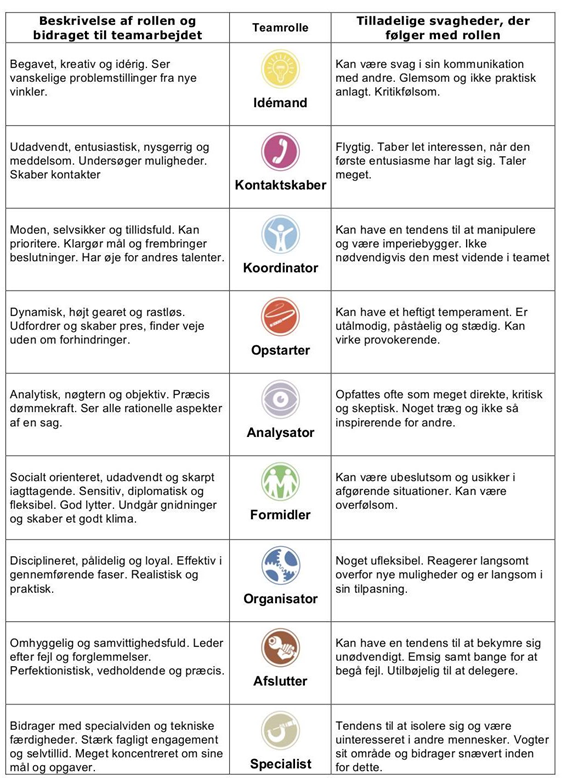
\includegraphics[width=11cm,height=14cm]{images/belbin teamroller.png}
\caption{Team Roller}
\label{fig:roller}
\end{center}
\end{figure}
\\ Engelske betegnelser
\begin{itemize}
\item Idémand: Plant
\item Kontaktskaber: Resource investigator
\item Koordinator: Co-ordinator
\item Opstarter: Shaper
\item Analysator: Monitor - Evaluator
\item Formidler: Teamworker
\item Organisator:  Implementer
\item Afslutter: Completer - Finisher Specialist: Specialist
\end{itemize}
\item Verbale kendetegn ved Belbin teamroller
\\ Jo mere hver enkelt udfører sin bedste teamrolle jo bedre samarbejde. Men det er ikke altid nemt at identificere sig med en teamrolle, og det er ikke altid at den enkelte signalerer sin teamrolle så tydeligt, at andre kan aflæse den. Verbale kendetegn kan bruges til at tydeliggøre ens teamrolle-identitet for andre. se figuren ~\ref{fig:kendetegn}:
\begin{figure}[h]
\begin{center}
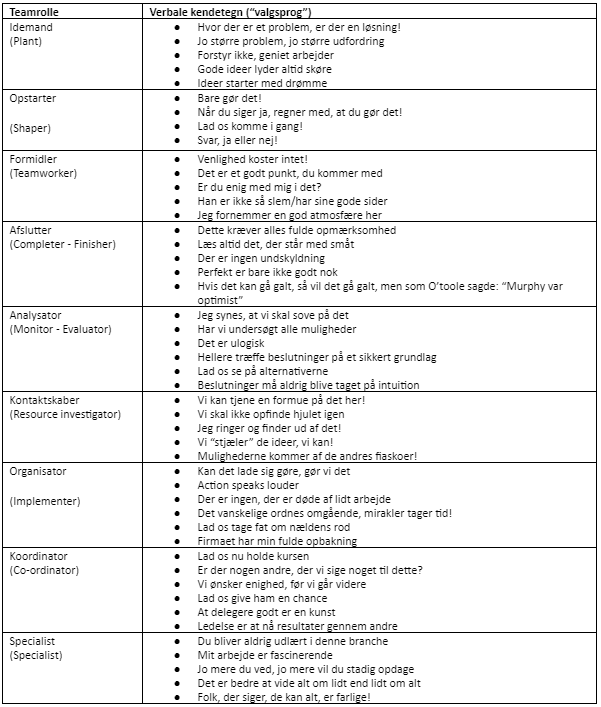
\includegraphics[width=13cm,height=18cm]{images/verbale kendetegn.png}
\caption{Verbale Kendetegn}
\label{fig:kendetegn}
\end{center}
\end{figure}
\item DSMI Den Syddanske Model for Ingeniøruddannelser (2015), Læringsmiljøet. 
\\ \url{https://tek-teach.sdu.dk/index.php?page=da-DSMI}
\\ tilgået 03. august 2022. 
\item 5 skriveregler 
\\ \url{https://skrivekrampen.blogspot.com/2017/10/george-orwells-6-regler-til-sprog.html} 
\\ tilgået 3. august 2022 
\item \url{https://mitsdu.dk/da/bibliotek} 
\item Kanban board \url{https://kanbantool.com/personal-kanban-board}
\item AU Studypedia: Skriv opgaven! \url{https://studypedia.au.dk/skriv-opgaven}
\item AU Studypedia: Feedback \url{https://studypedia.au.dk/gruppearbejde/feedback}
\end{itemize}
\AtEndDocument{
\section{Appendix 1: Kapitel 1 Problemorienteret projektarbejde}\label{sec:Kap1}
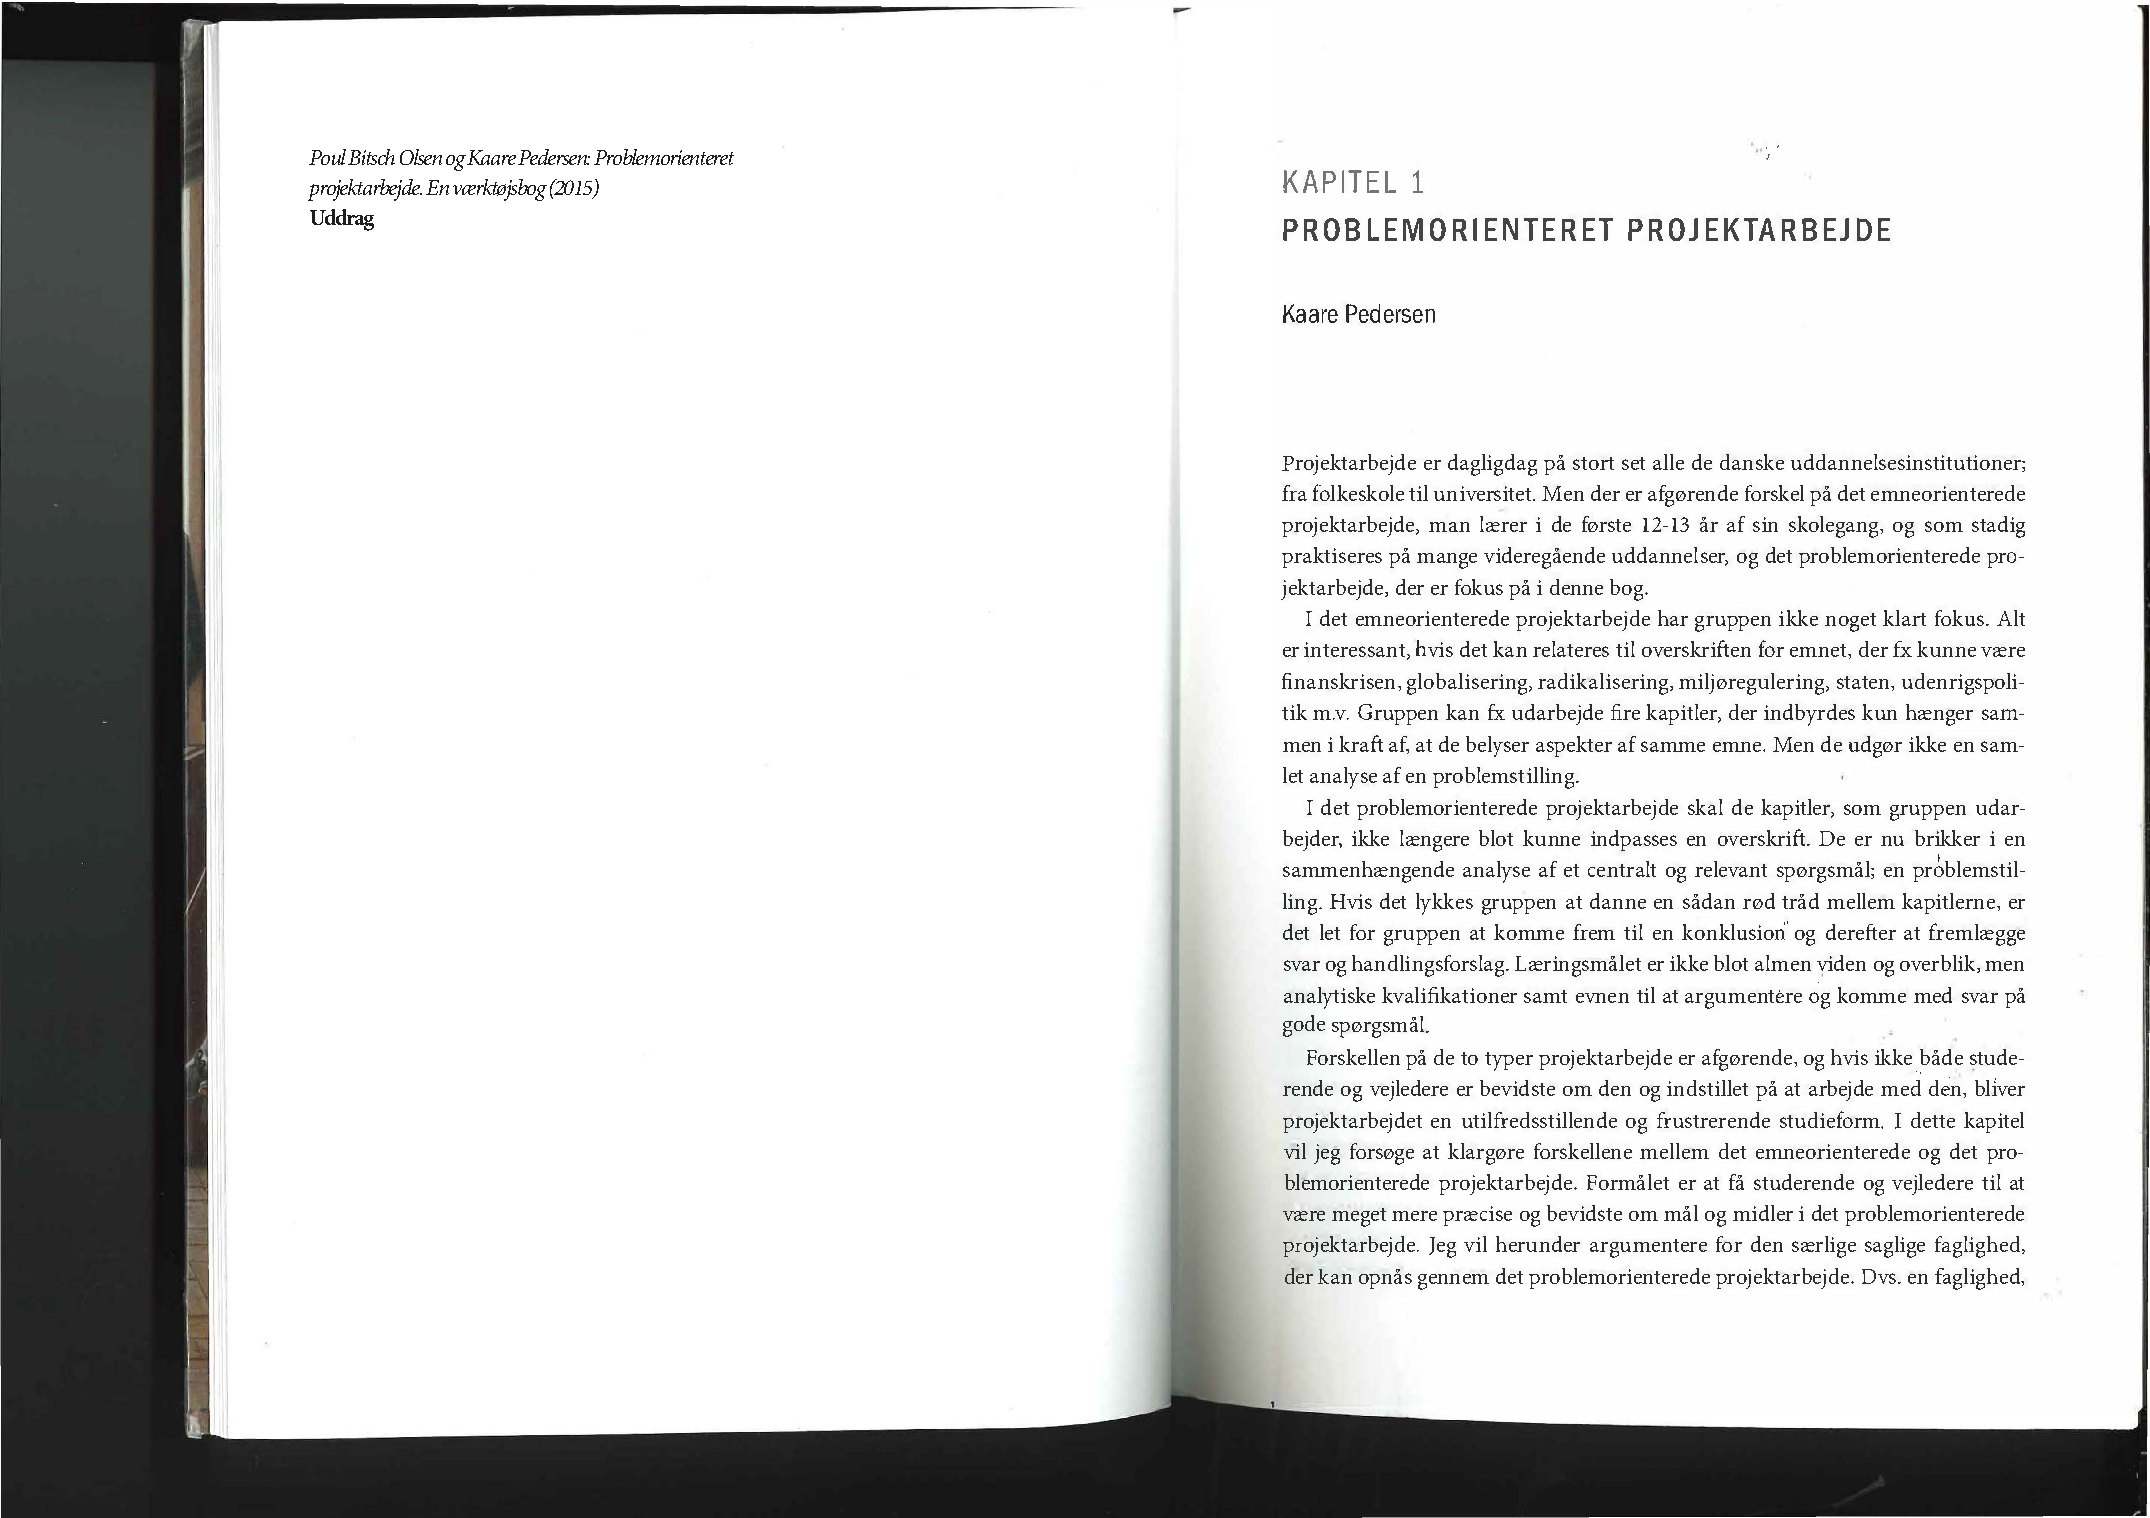
\includepdf[pages=-,pagecommand={}]{pdfs/Kap1.pdf}
\section{Appendix 2: Kapitel 8 Styrk projektarbejdet}\label{sec:Kap8}
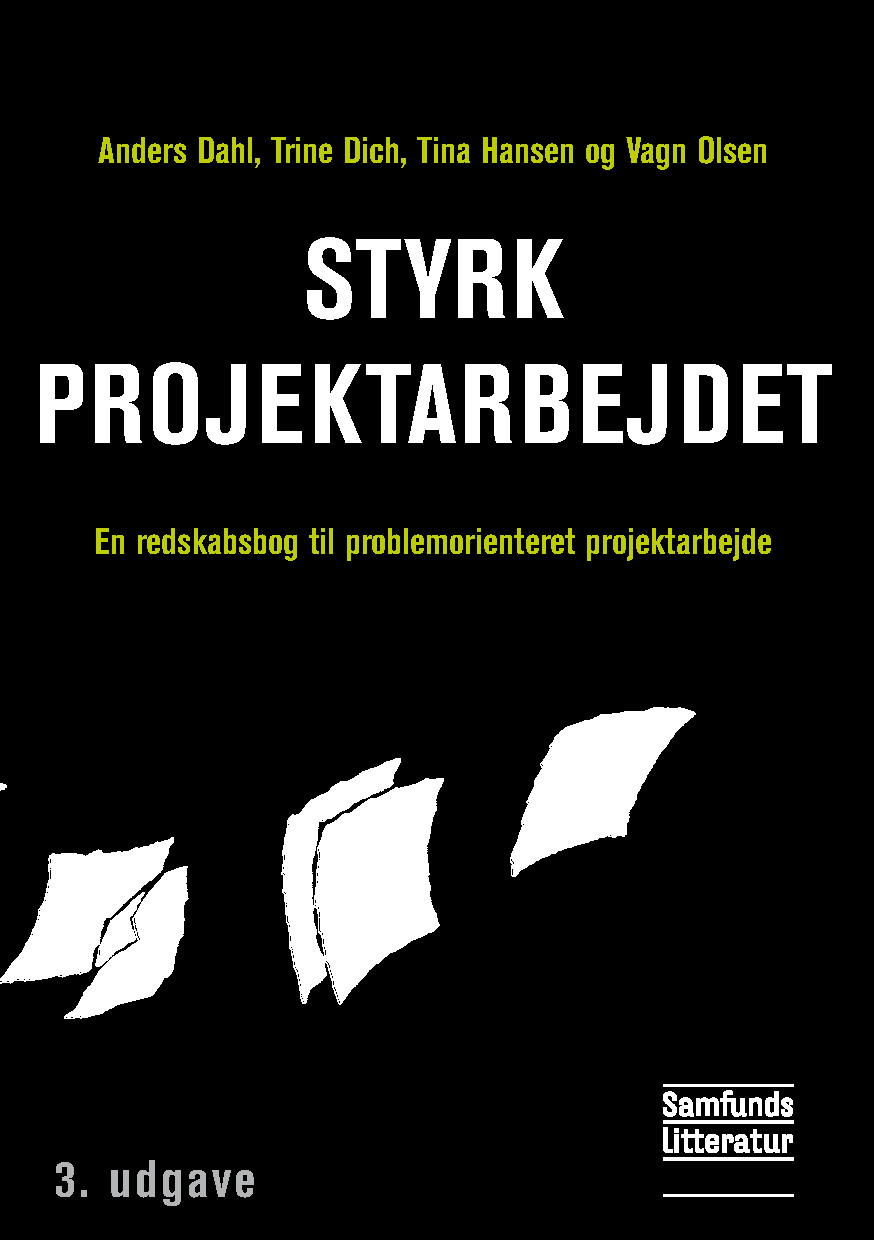
\includepdf[pages=-,pagecommand={}]{pdfs/Kap8.pdf}
}

\end{document}
